\documentclass{beamer}
% Nächstes Auskommentieren um jedes \pause zu 'deaktivieren'!
%\documentclass[handout]{beamer}

\usepackage{talk_BeamerColor}

\usepackage[pantoneblack7,english]{talk_wwustyle_LA}

\usepackage[ngerman]{babel}
\usepackage[utf8]{inputenc}
\usepackage[T1]{fontenc}
\usepackage{lmodern}
% --- Paket um Grafiken im Dokument einbetten zu koennen
\usepackage{graphicx}
\usepackage{caption}
\usepackage{subfigure}
\usepackage{wrapfig}
\usepackage{tikz}

% --- Pakete fuer mathematischen Textsatz
\usepackage{amsmath}
\usepackage{amssymb}
\usepackage{empheq}
\usepackage{dsfont}		
\usepackage{amstext}
\usepackage{amsfonts}
\usepackage{amsthm}
\usepackage{wasysym}

% --- Paket erweitert deutlich die Verwendung von Farben aus dem Paket 'graphicx'
\usepackage{color}

% --- Paket um Quellcode sauber zu formatieren
\usepackage{listings}

% --- Darstellung von Pseudocode und mehr (algorithmicx packages)
\usepackage{algorithm}
\usepackage{algpseudocode}

%% Physikalisches
\usepackage{nicefrac}
\usepackage{units}
\usepackage{siunitx}
\sisetup{
  inter-unit-product 	=	$\cdot$,
  fraction-function   	= 	\nicefrac,
  load-configurations 	= 	abbreviations,
  per-mode            	= 	fraction,
  separate-uncertainty	=	true,
  output-decimal-marker	=	{.}
  }   
\usepackage{isotope}

%% Aufgabenverwaltung
\usepackage[textwidth=2cm,% Breite der Todo-Eintr�ge
            textsize=footnotesize,% Schriftgr��e der Eintr�ge
            english,% deutsche Beschriftungen
            shadow,% Schlagschatten f�r Boxen (weils so h�bsch ist)
            colorinlistoftodos]{todonotes}% farbige Markierungen f�r unterschiedliche Aufgabentypen
\newcommand{\detail}[1]{\todo[color=Green,inline]{detail: #1}~}% Details k�nnten hinzugef�gt werden
\newcommand{\litcheck}[1]{\todo[color=LightSteelBlue,inline]{refcheck: #1}~}% muss noch einmal �berpr�ft werden
\newcommand{\src}[1][]{\todo[color=Tomato,inline]{reference! #1}~}% Quelle fehlt

% % Zusätzliches:
\usepackage{braket}
\usepackage{epstopdf}
\usepackage{pgfpages}
\usepackage{csquotes}

\newlength{\halftextwidth}
\setlength{\halftextwidth}{\textwidth}
\divide\halftextwidth by 2

% --- Einstellungen

\author{NiMoNa (Abschlusspräsentation) SoSe 2016}
\title{Konnektivität im Gehirn}
%\institutelogo{Logo on title frame}
%\institutelogosmall{Logo on other frames}
\subtitle{Lutz Althüser, Tobias Frohoff-Hülsmann, Victor Kärcher,\\ Lukas Splitthoff, Timo Wiedemann\\ \vspace{0.25cm} Unterstützt durch: Christian Himpe}
\date[13.07.2016]{13. Juli, 2016}

% --- Beginn des Dokuments

\begin{document}

\begin{frame}[plain]
	  \maketitle
\end{frame}

\begin{frame}{Überblick}
	\tikz[remember picture,overlay]
	\node at ([xshift=-2.5cm,yshift=-5cm]current page.north east)
	{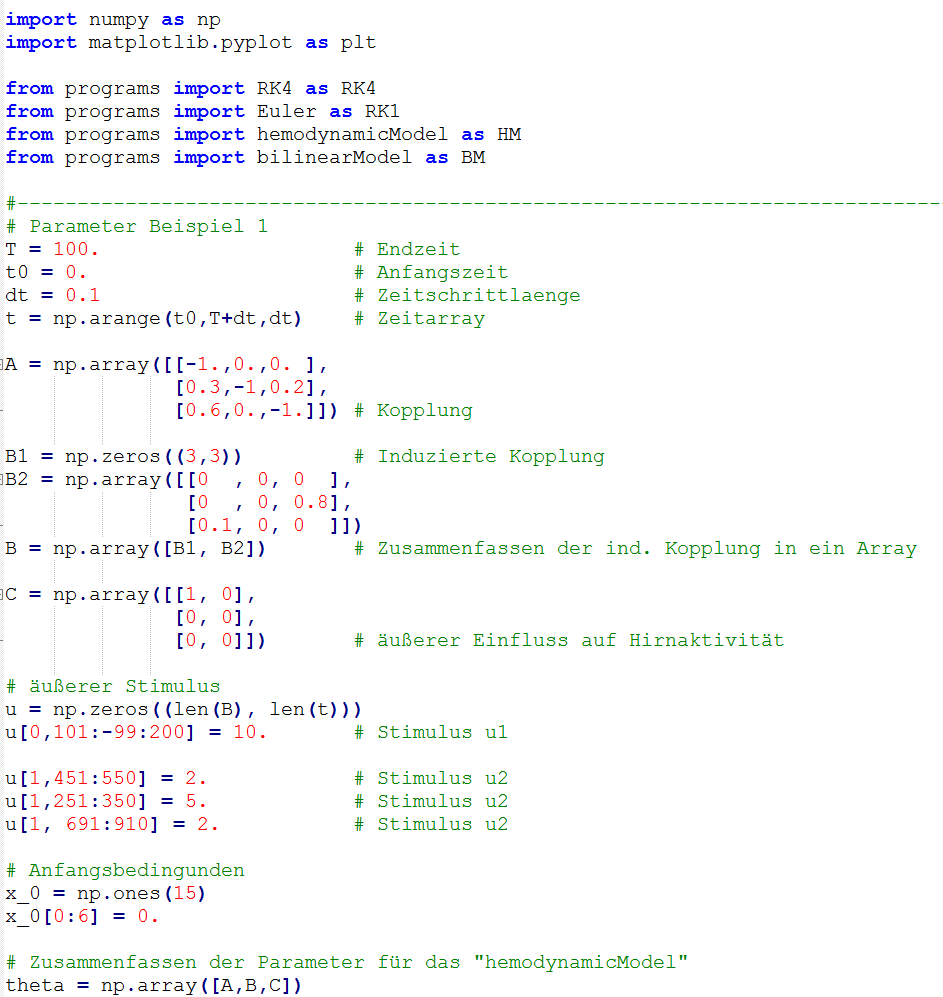
\includegraphics[height=7cm,angle=-7.5,keepaspectratio]{res/toc.png}};
	\tableofcontents
	  
\end{frame}

\section{DCM für fMRI - Rückblick}
\begin{frame}[t]{\underline{D}ynamic \underline{C}ausal \underline{M}odelling für fMRI}
	\begin{columns}
		\column[t]{8.3cm}
		\vspace{-0.7 cm}
		\begin{itemize}
			\item \textit{Ziel:} \\Modellierung von Interaktionen in einem neuronalen Netzwerk\\[0.3cm]
			\item \textit{Ansatz:} \\Modellierung neuronaler Zustandsentwicklung mithilfe einer Taylorreihen-Näherung\\$ \longrightarrow $ \textit{Netzwerk-Modell}\\[0.3cm]
			\item \textit{Vergleichbarkeit mit Experiment:} \\ Hämodynamisches Modell:\\ Basierend auf Variation des Blutvolumens und des desoxygenierten Hämoglobins\\$ \longrightarrow $ \textit{Observablen-Modell}
		\end{itemize}
		\column[t]{4.5cm}
			\vspace{-0.3 cm}
			\begin{figure}
				\centering
				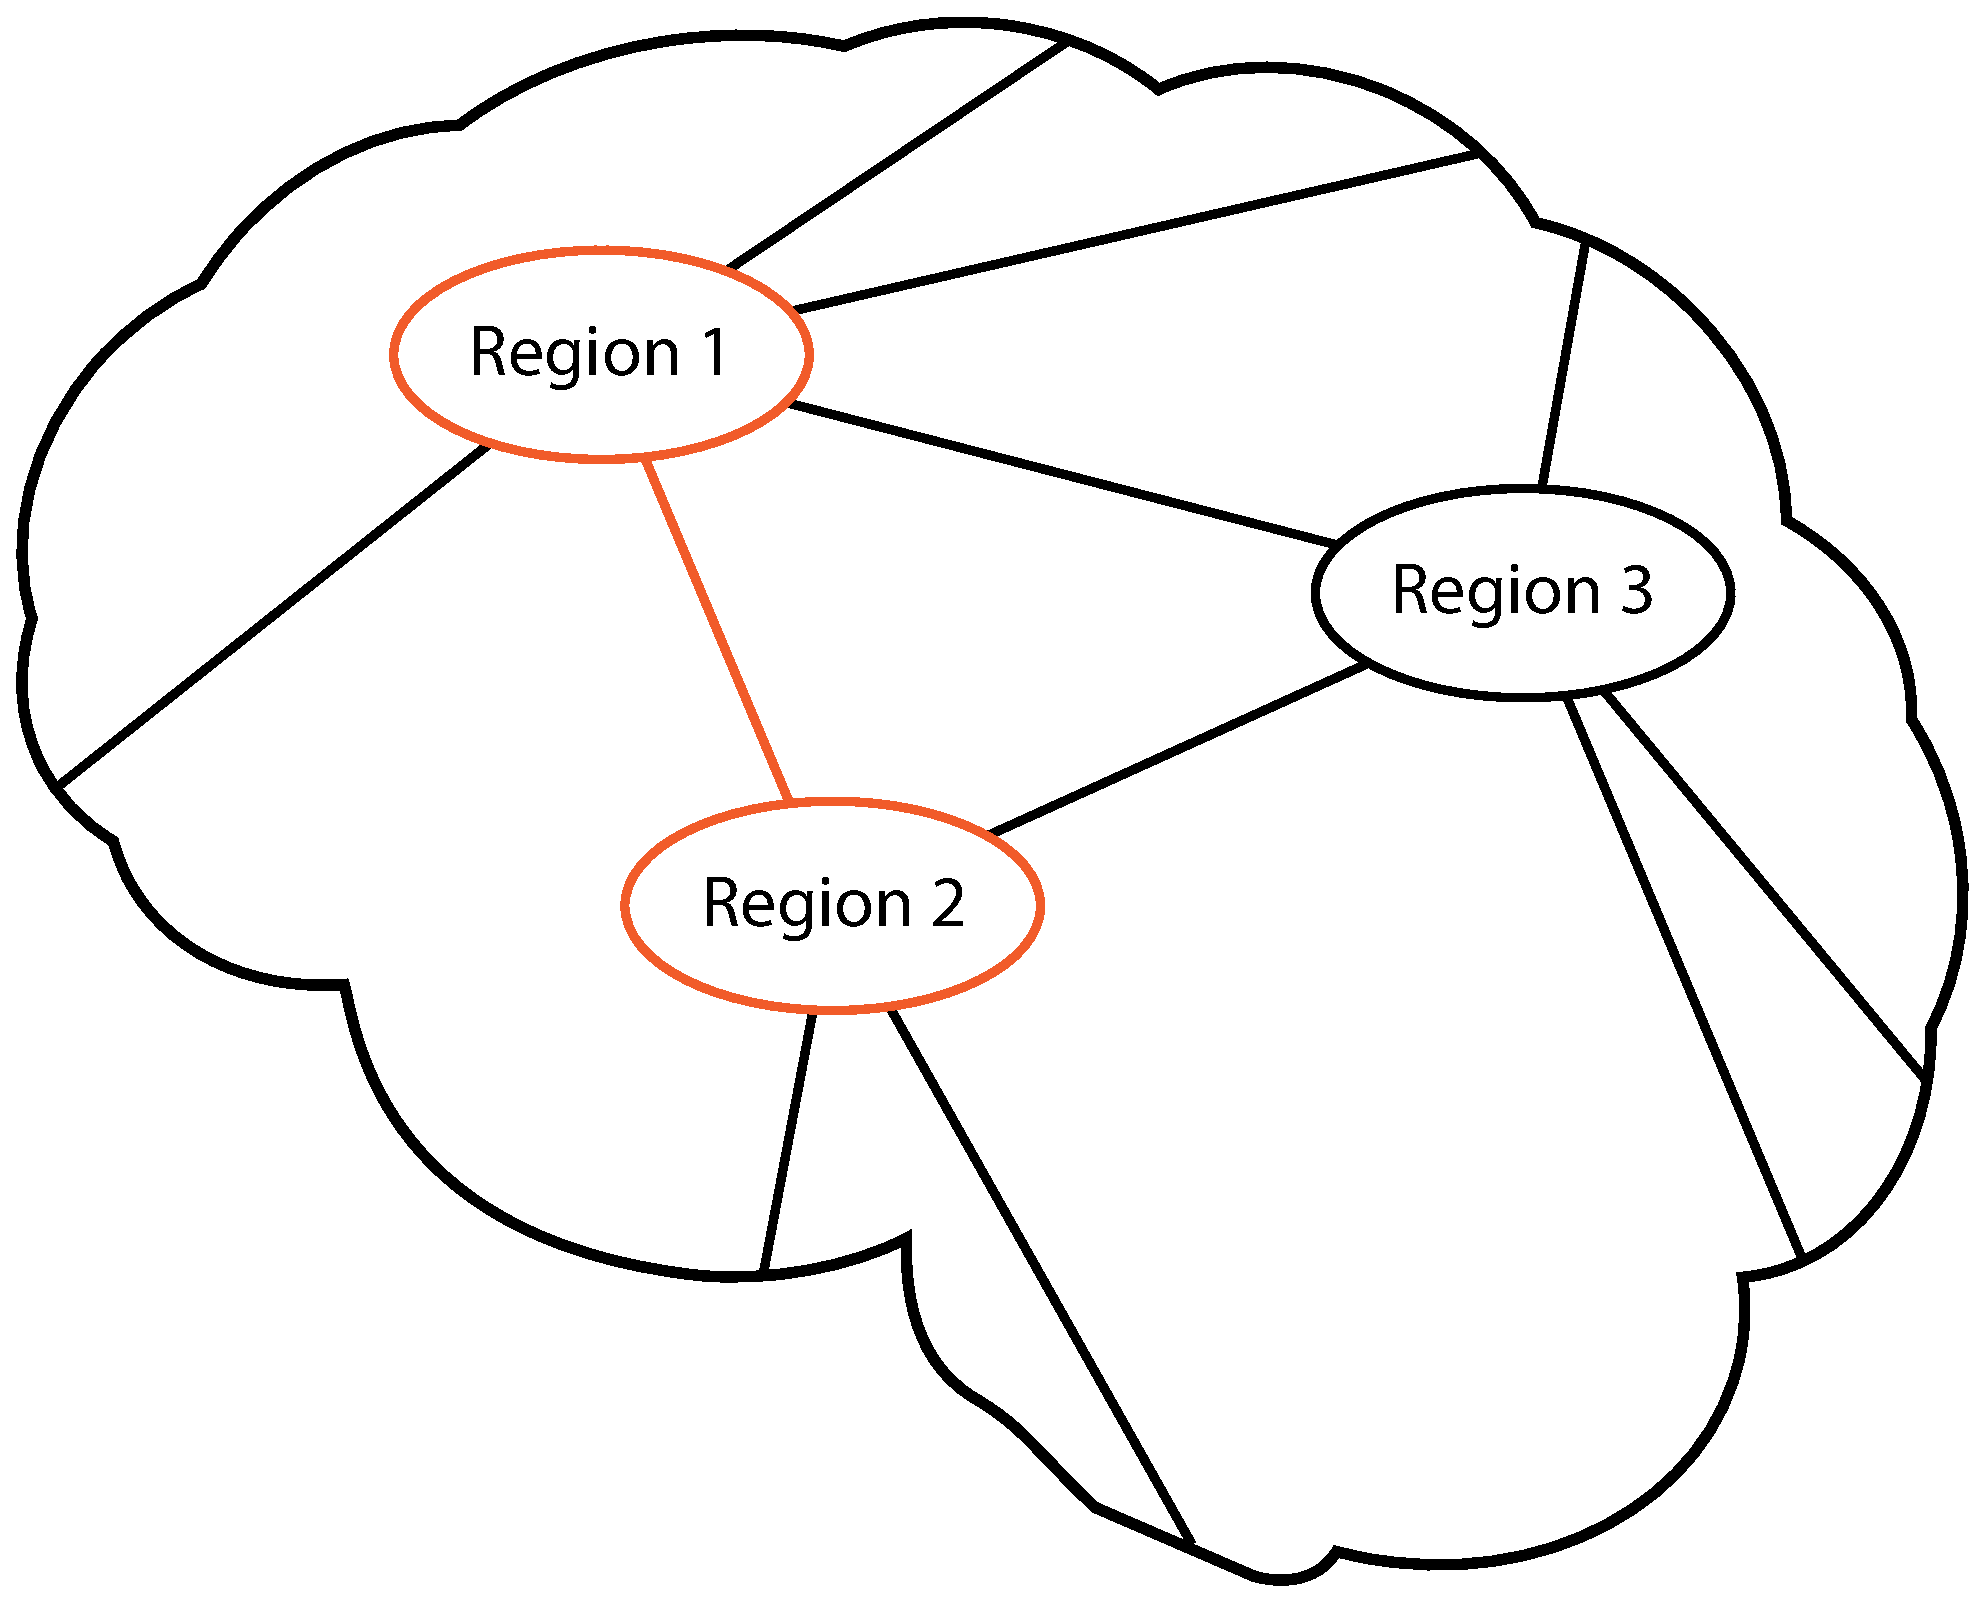
\includegraphics[width=0.9\linewidth]{res/brain_01.eps}
				\\ {\footnotesize Interaktion zwischen}\\ {\footnotesize verschiedenen Hirnregionen}
			\label{fig:brain_01}
		\end{figure}
	\end{columns}

\end{frame}
%%%%%%%%%%%%%%%%%%%%%%%%%%%%%%%%%%%%%%%%%%%%%%%%%%%%%%%%%%%%%%%%%%%%%%%%%%%%%%%%%%%%%%%%%%%%%%
\begin{frame}{Bilineares Netzwerk-Modell}
	\begin{columns}
		\column[t]{5.5cm}
		\vspace{-20pt}
		\begin{figure}
			\centering
			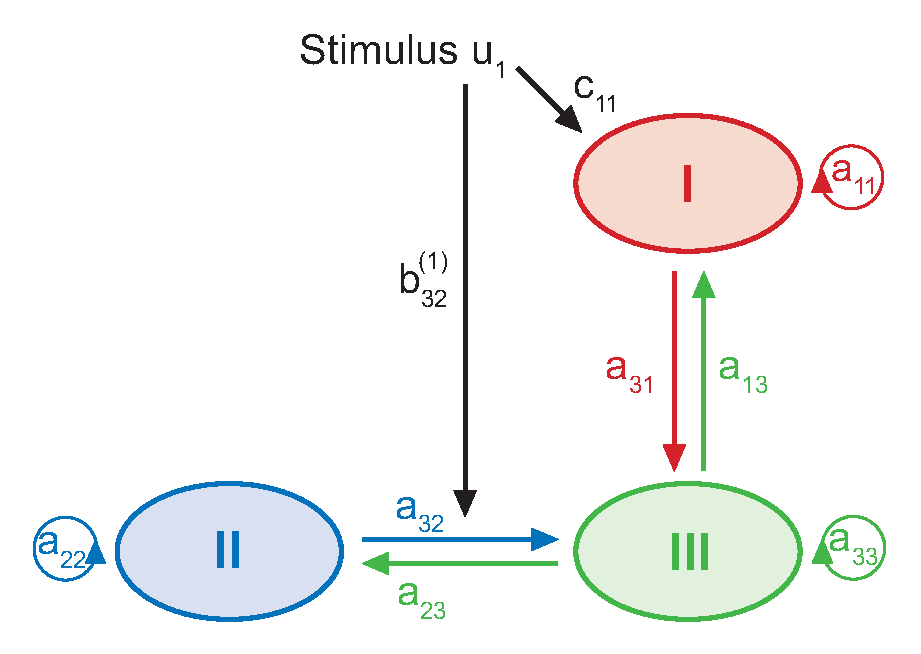
\includegraphics[width=0.8\linewidth]{res/160711bilinearExpl.eps}
		\end{figure}
		\centering
		\vspace{-10pt}
		\scalebox{.6}{
			\begin{minipage}{1.3\textwidth}
				\begin{block}{Mathematische Beschreibung}
					\begin{itemize}
						\item A: feste Verknüpfung der Hirnregionen
						\item B: Einfluss des Inputs auf Konnektivität
						\item C: Einfluss des Inputs auf neuronale Aktivität der Hirnregionen						
					\end{itemize}
				\end{block}
			\end{minipage}
		}
		\column[t]{9cm}
		
		\scalebox{.8}{
			\begin{minipage}{\textwidth}

				\begin{flalign*}
					\dot{z}(t)&=f(z(t),u(t)) &\\
					&\approx f(0,0)+\frac{\partial f}{\partial z}z+\frac{ \partial f}{\partial u} u + \frac{\partial^2 f}{\partial z \partial u}zu &\\
				\end{flalign*}
			\end{minipage}
		}
		
		\scalebox{.8}{
			\begin{minipage}{\textwidth}
			\colorbox{maincolor!10}{
				$
				\dot{z}(t)=A\cdot z+\sum_{j}u_jB^j\cdot z+C\cdot u
				$
			}
			\end{minipage}

		}	
		\scalebox{.8}{
			\begin{minipage}{\textwidth}		
				\vspace{16pt}
				$ A=
				\begin{pmatrix}
				a_{11} 	& 0 	 & a_{13}\\
				0		& a_{22} & a_{23}\\
				a_{31} 	& a_{32} & a_{33}
				\end{pmatrix}
				$
				\hspace{5pt} 
				$ B^{(1)}=
				\begin{pmatrix}
				0	& 0 			& 0\\
				0 	& 0 			& 0\\
				0	& b_{32}^{(1)} 	& 0
				\end{pmatrix}
				$
				\\
				\\
				\\					
				$ C=
				\begin{pmatrix}
				c_{1}	\\
				0 	\\
				0	 
				\end{pmatrix}
				$										
			\end{minipage}
		}				
	\end{columns}
	
	\centering
	\vspace{5pt}
	$ \rightarrow $ Neuronale Aktivität $ \leftrightarrow $ Konnektivität
\end{frame}

%%%%%%%%%%%%%%%%%%%%%%%%%%%%%%%%%%%%%%%%%%%%%%%%%%%%%%%%%%%%%%%%%%%%%%%%%%%%%%%%%%%%%%%%%%%%%%

\section{Nichtlineare Erweiterung des Modells}
\begin{frame}{Nichtlineare Erweiterung}
	\vspace{-0.4cm}
	\begin{columns}
		\column[t]{5.5cm}
		\vspace{-20pt}
		\begin{figure}
			\centering
			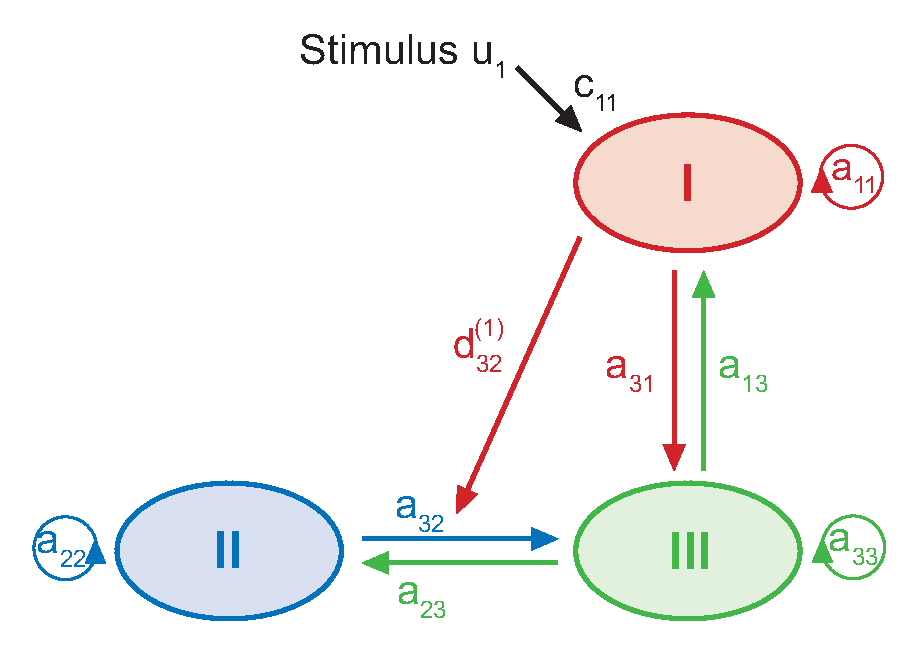
\includegraphics[width=0.8\linewidth]{res/160711nichtlinearExpl.eps}
		\end{figure}
		\centering
		\vspace{-10pt}
		\scalebox{.6}{
			\begin{minipage}{1.3\textwidth}
				\begin{block}{Mathematische Beschreibung}
					\begin{itemize}
						\item A: feste Verknüpfung der Hirnregionen
						\item B: Einfluss des Inputs auf Konnektivität
						\item C: Einfluss des Inputs auf neuronale Aktivität der Hirnregionen
						\item D: Einfluss der Regionen auf Konnenktivität						
					\end{itemize}
				\end{block}
			\end{minipage}
		}
		\column[t]{9cm}
		
		\scalebox{.8}{
			\begin{minipage}{\textwidth}
				
				\begin{flalign*}
				\dot{z}(t)&=f(z(t),u(t)) &\\
				&\approx f(0,0)+\frac{\partial f}{\partial z}z+\frac{ \partial f}{\partial u} u + \frac{\partial^2 f}{\partial z \partial u}zu + \textcolor{blue}{\frac{\partial^2 f}{\partial z^2} \frac{z^2}{2}}&\\
				\end{flalign*}
			\end{minipage}
		}
		
		\scalebox{.8}{
			\begin{minipage}{\textwidth}
				\colorbox{maincolor!10}{
					$
					\dot{z}(t)=A\cdot z+\sum_{j}u_jB^j\cdot z+C\cdot u+\textcolor{blue}{\frac{1}{2}\sum_{i}z_{i}D^{i}\cdot z}
					$
				}
			\end{minipage}
			
		}	
		\scalebox{.8}{
			\begin{minipage}{\textwidth}		
				\vspace{16pt}
				$ A=
				\begin{pmatrix}
				a_{11} 	& 0 	 & a_{13}\\
				0		& a_{22} & a_{23}\\
				a_{31} 	& a_{32} & a_{33}
				\end{pmatrix}
				$
				\hspace{5pt} 
				$ B^{(1)}=
				\begin{pmatrix}
				0	& 0 			& 0\\
				0 	& 0 			& 0\\
				0	& \textcolor{blue}{0}			 	& 0
				\end{pmatrix}
				$				
				\\
				\\
				\\					
				$ C=
				\begin{pmatrix}
				c_{1}	\\
				0 	\\
				0	 
				\end{pmatrix}
				$	
				\hspace{58pt}
				$ \textcolor{blue}{ D^{(1)}=
				\begin{pmatrix}
				0	& 0 			& 0\\
				0 	& 0 			& 0\\
				0	& d_{32}^{(1)} 	& 0
				\end{pmatrix}
				}$									
			\end{minipage}
		}				
	\end{columns}
	
	
\end{frame}

\begin{frame}{Simulation eines 4-Regionen-Systems}
 \centering
 \colorbox{maincolor!10}{\underline{Idee}: \quad Autoregulation einer Region}
	\begin{figure}
		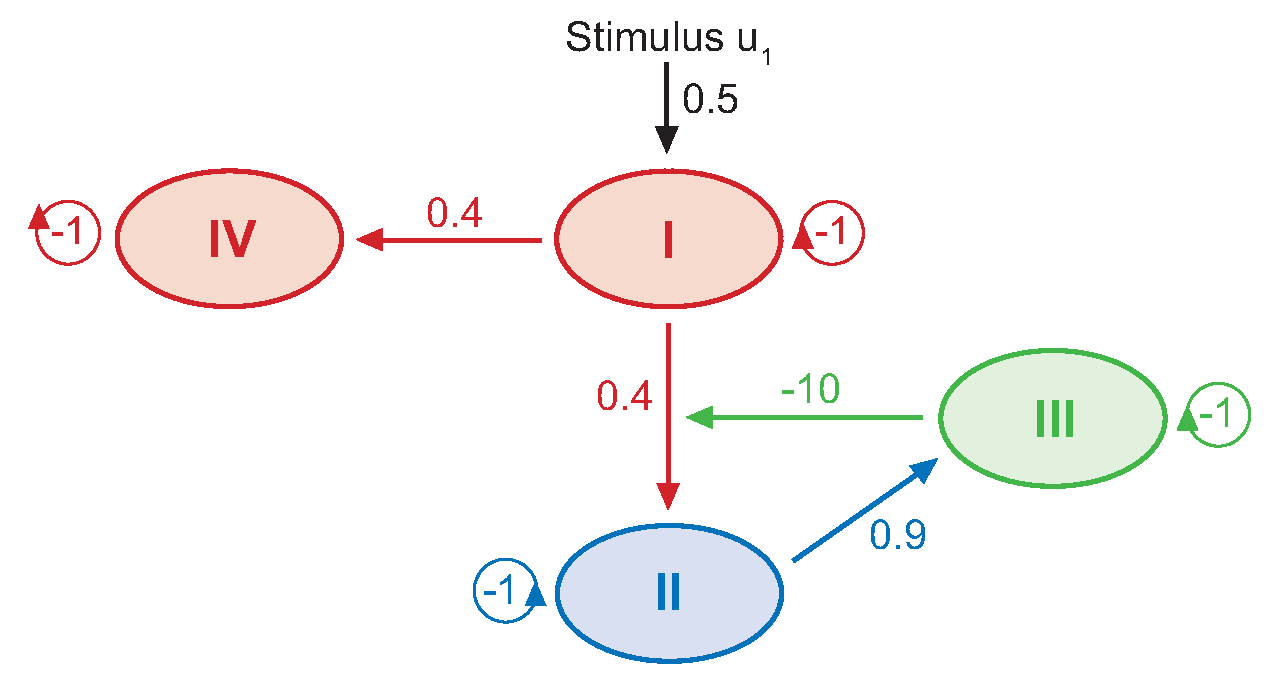
\includegraphics[width=0.8\textwidth]{res/160711Autoregulation1.eps}
	\end{figure}
\end{frame}

\begin{frame}{Simulation eines 4-Regionen-Systems}
	\begin{figure}
		\vspace*{-0.33cm}
		\centering
		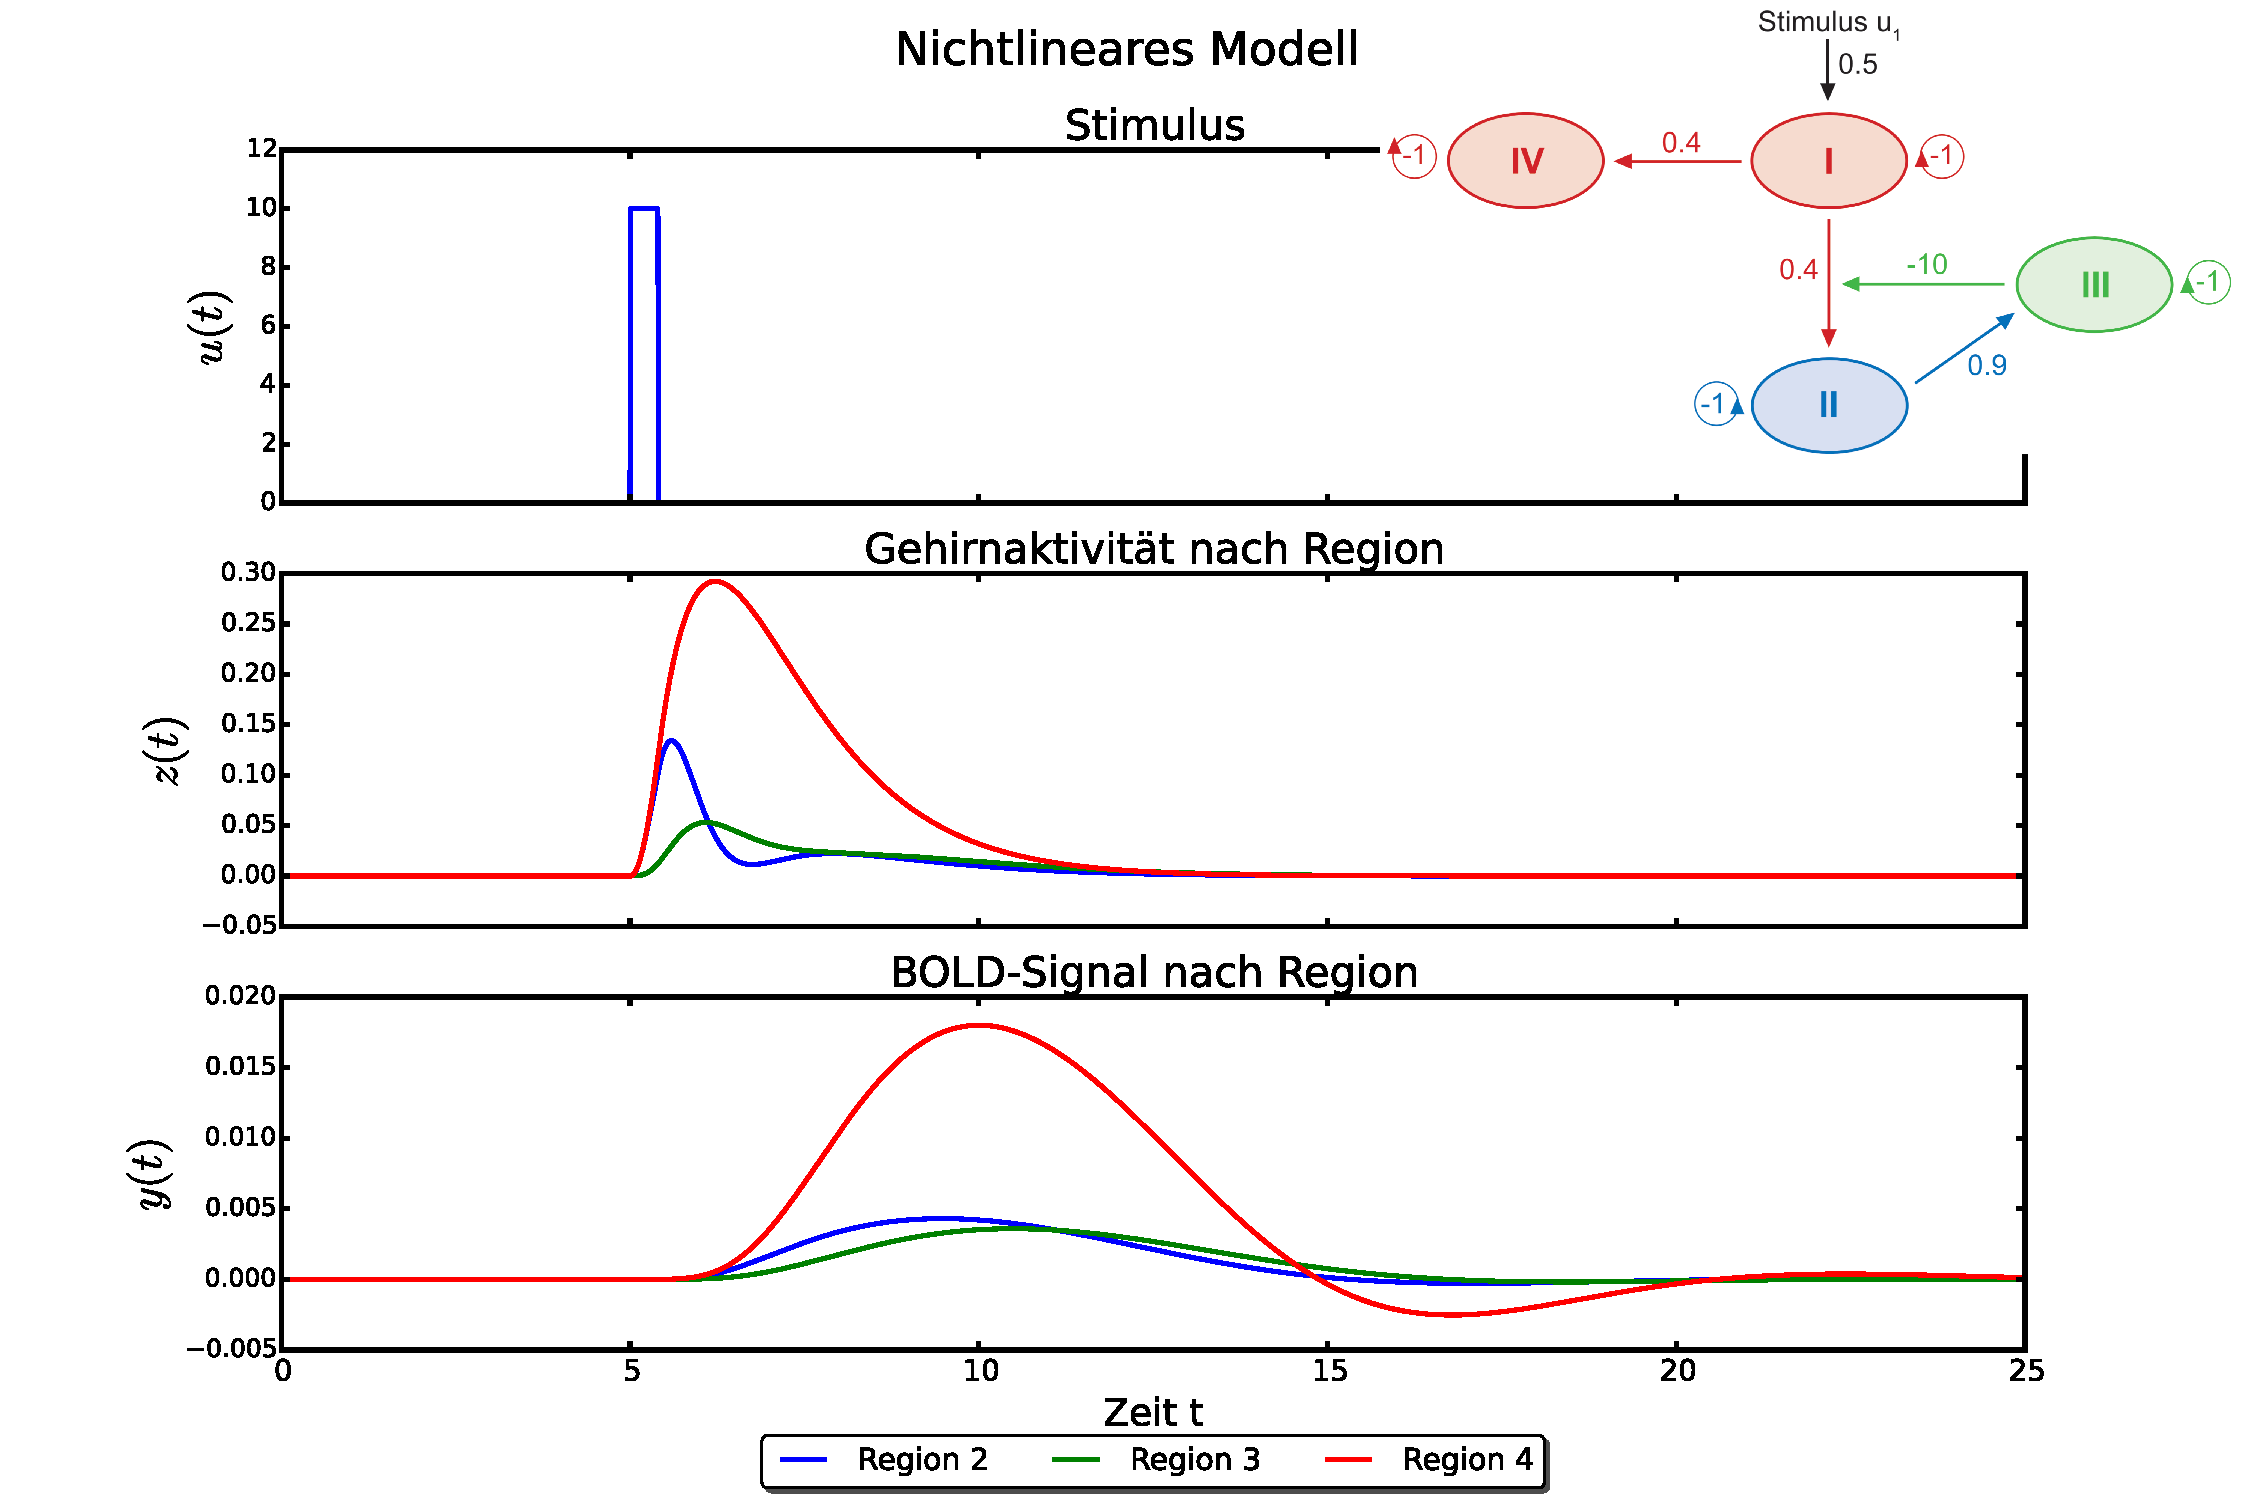
\includegraphics[width=0.975\textwidth]{res/hemodynamicExample1.pdf}
	\end{figure}
\end{frame}

\begin{frame}{Simulation eines 4-Regionen-Systems}
 \centering
 \colorbox{maincolor!10}{\underline{Frage}: \quad Selbiges Resultat ohne nichtlineare Erweiterung möglich?}
	\begin{figure}
		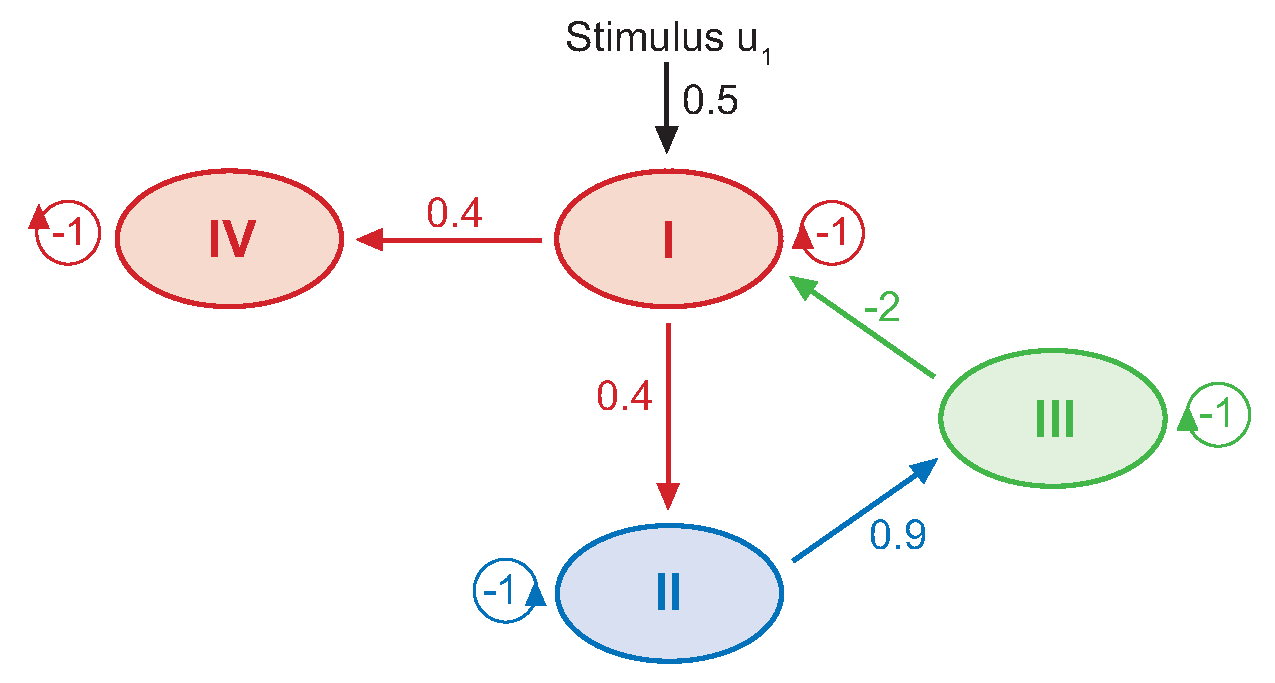
\includegraphics[width=0.8\textwidth]{res/160711Autoregulation2.eps}
	\end{figure}
 \colorbox{maincolor!10}{\underline{Problem}: \quad Einfluss auf weitere Region}
\end{frame}

\begin{frame}{Simulation eines 4-Regionen-Systems}
	\begin{figure}
		\vspace*{-0.33cm}
		\centering
		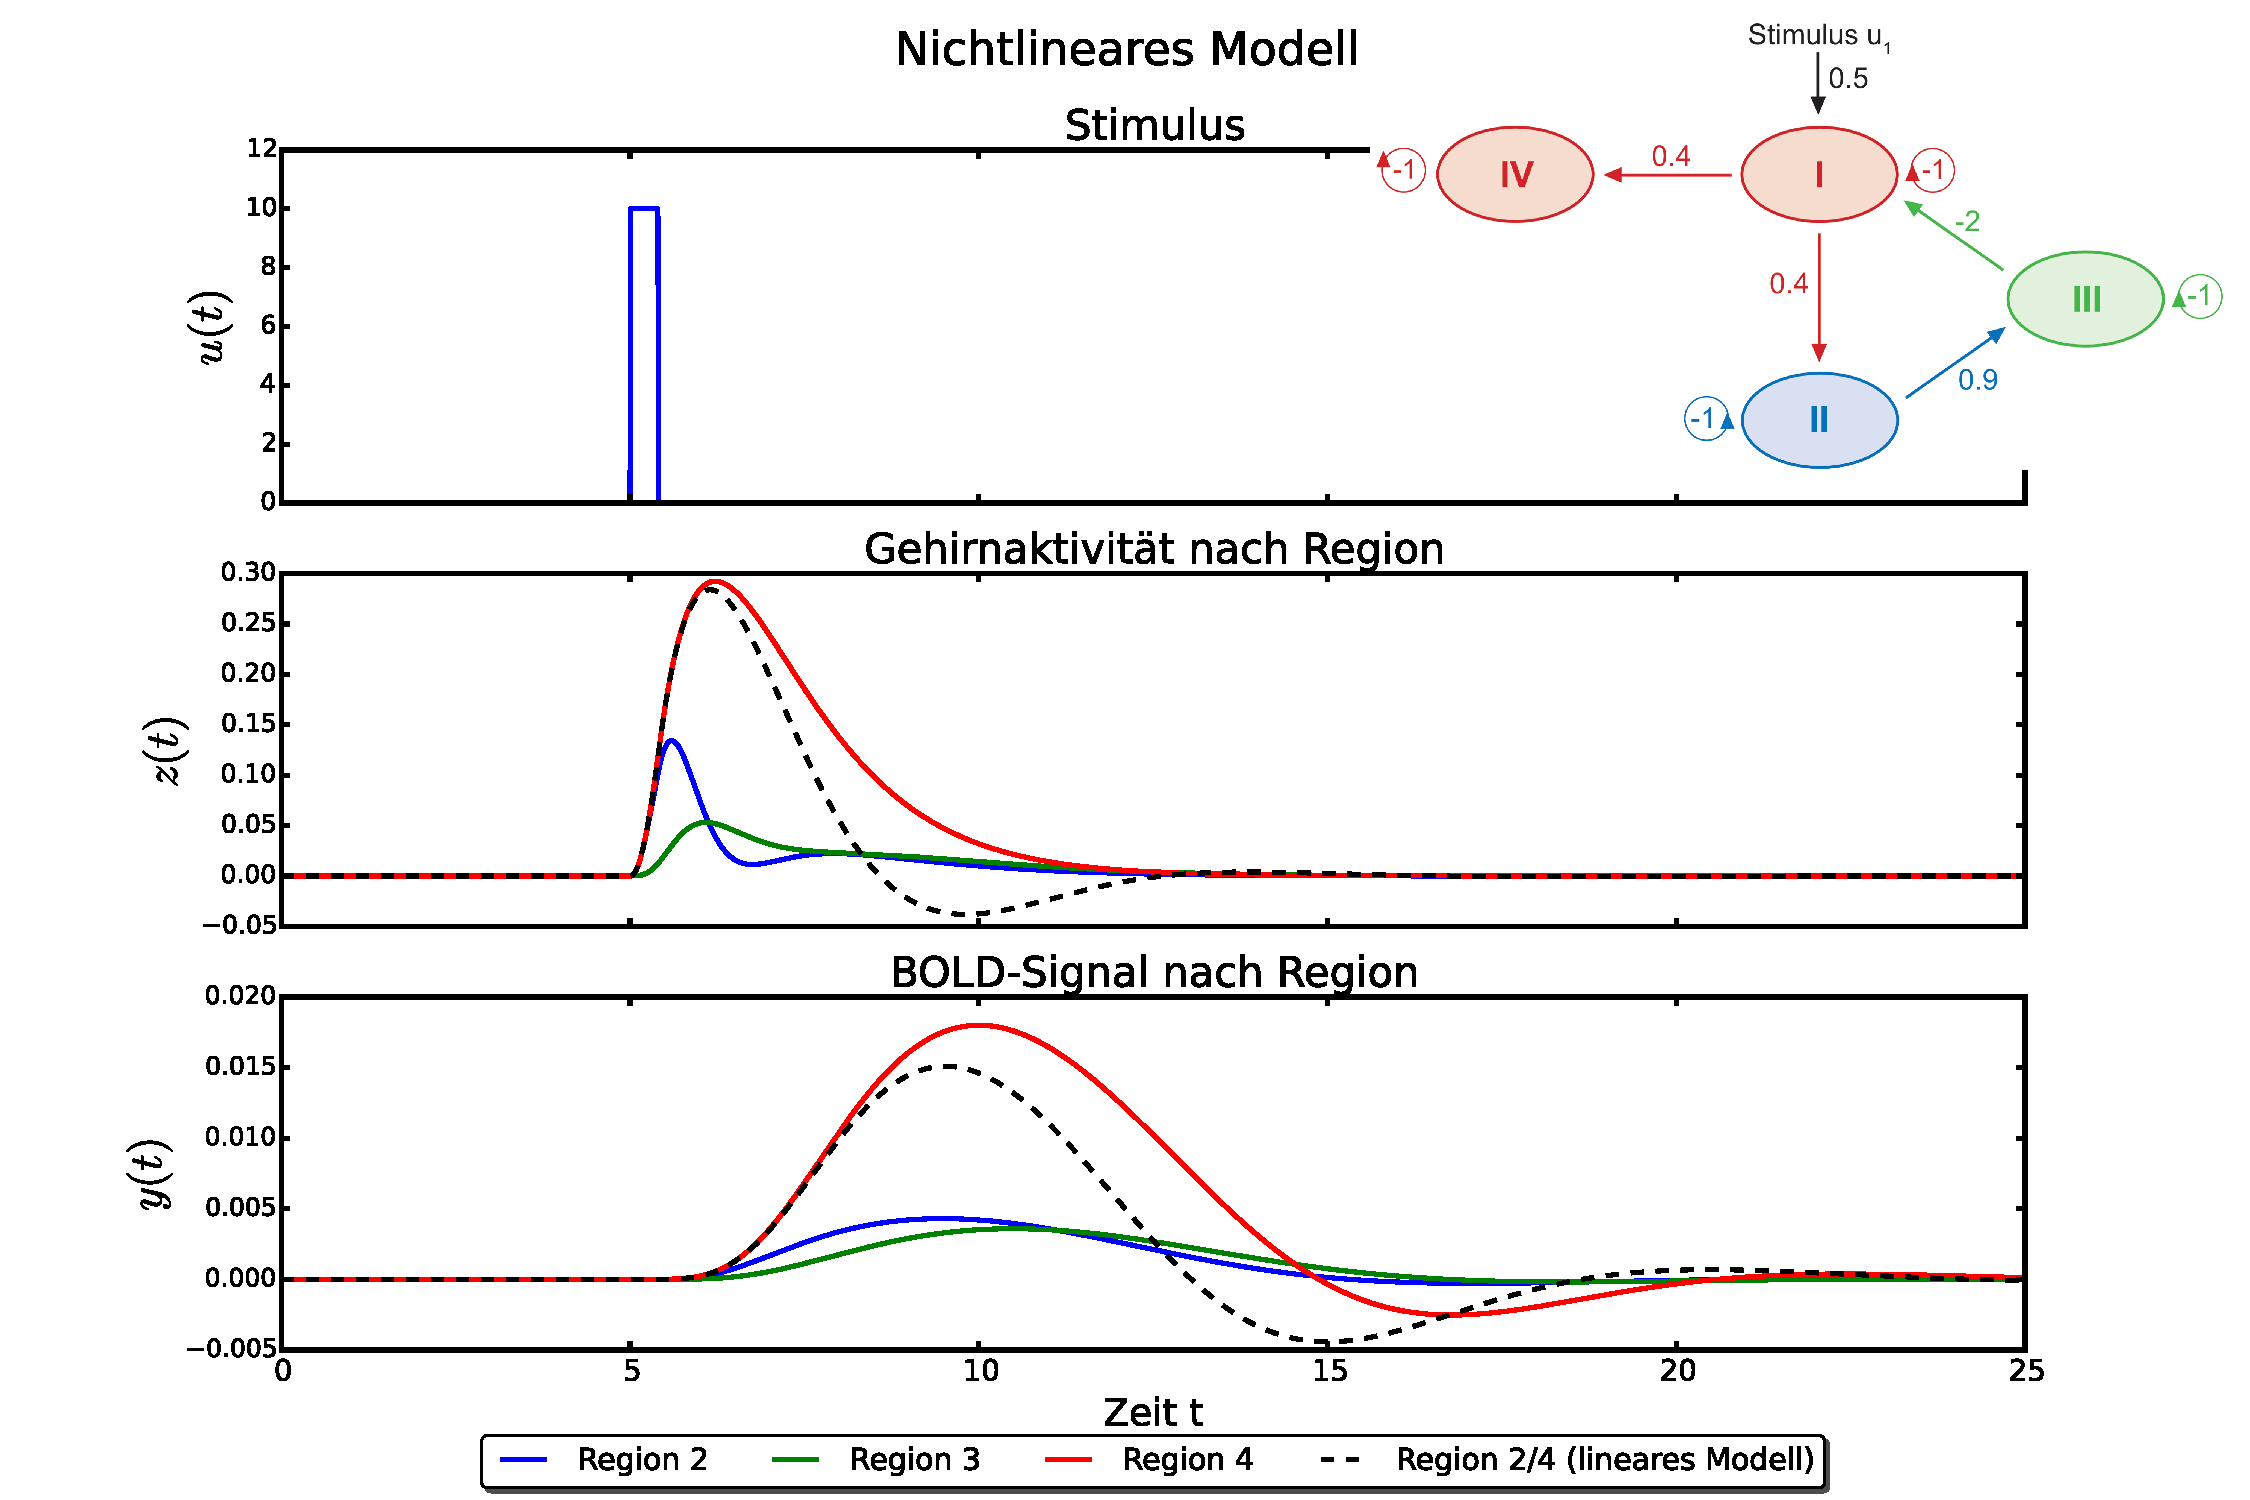
\includegraphics[width=0.975\textwidth]{res/hemodynamicExample2.pdf}
	\end{figure}
\end{frame}

%%%%%%%%%%%%%%%%%%%%%%%%%%%%%%
% 				EEG
%%%%%%%%%%%%%%%%%%%%%%%%%%%%%%
\section{EEG-Modell}
\begin{frame}{EEG}
\textbf{EEG = Elektroenzephalografie}
\begin{figure}
\centering
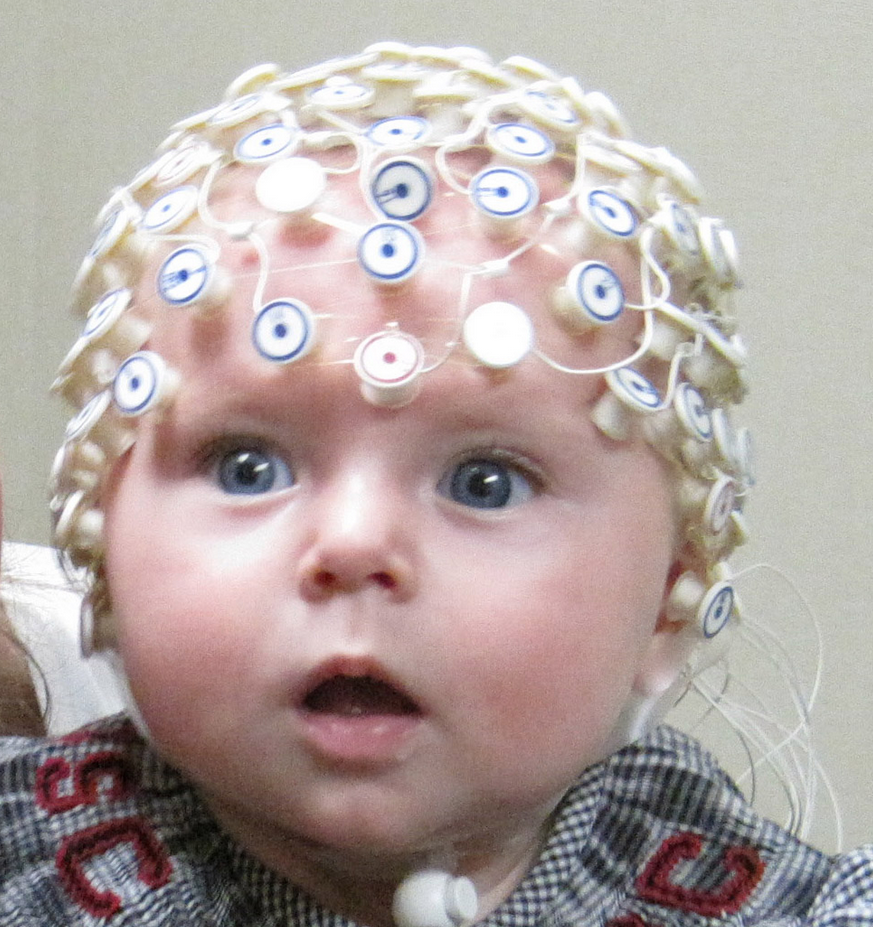
\includegraphics[scale=0.3]{res/EEGbaby.png}
\end{figure}
\end{frame}

\begin{frame}{Konzeptioneller Vergleich von fMRI- zu EEG-Modell}
\begin{tabular}{| c | c |}
\hline
\textbf{fMRI-Modell} & \textbf{EEG-Modell} \\
\hline
Verknüpfung einzelner Neuronen & Verknüpfung von Gehirnbereichen \\
&  und Subregionen untereinander \\
\hline
Taylorentwicklung & Eingangs- und \\
&  Ausgangsoperatoren \\
\hline
Gehirnaktivität = abstrakte Größe & direktes Modell für \\
biologisches Modell nötig & Potentiale und Potentialflüsse\\
\hline
\end{tabular}
\end{frame}

\begin{frame}{Das EEG-Modell}
\begin{figure}
\centering
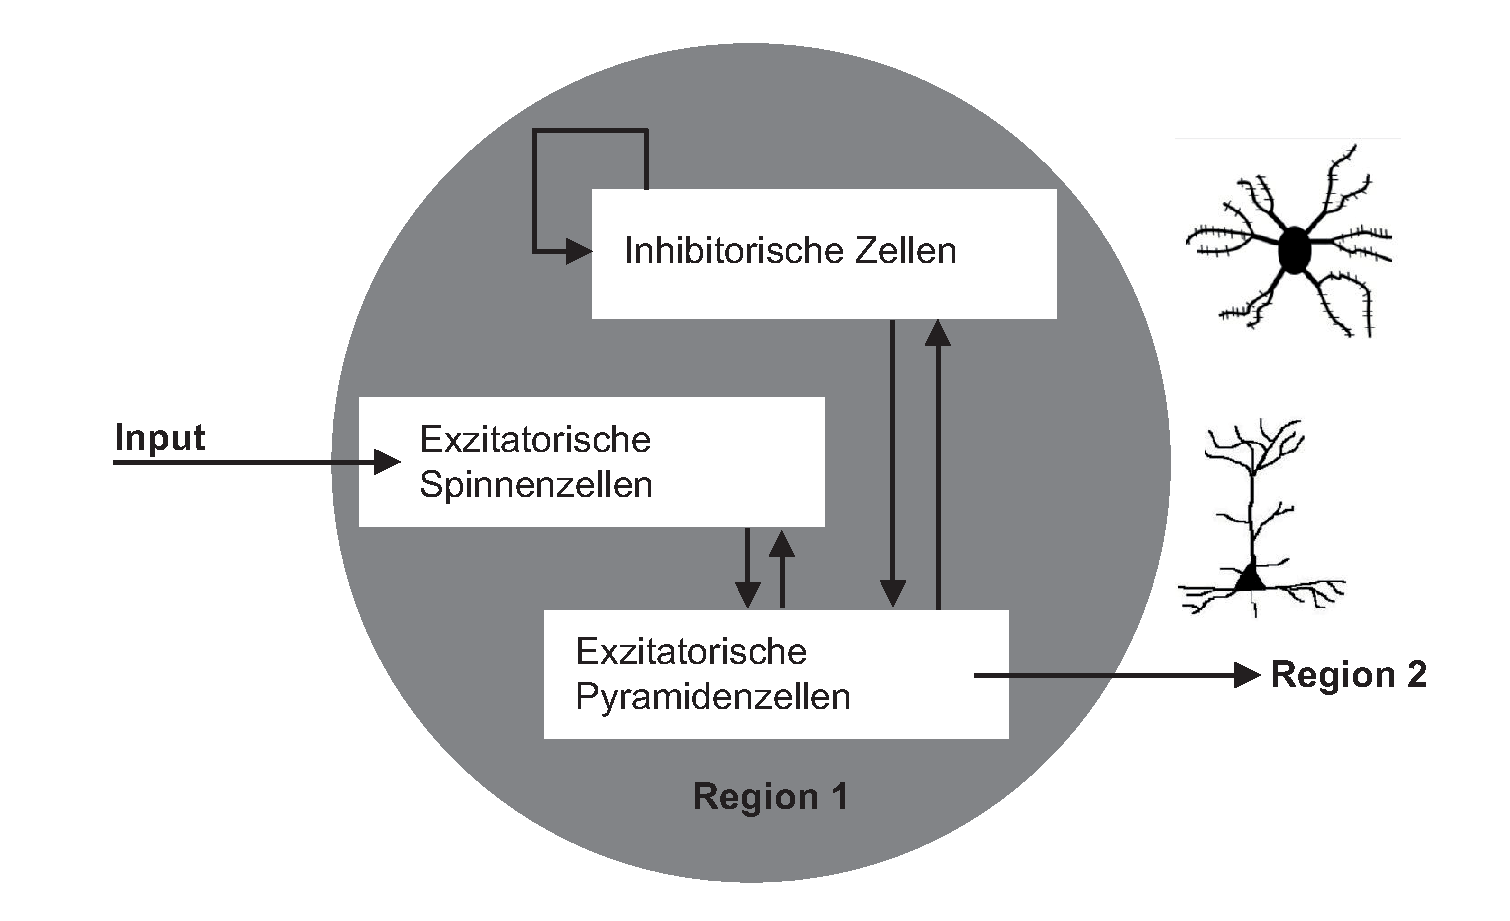
\includegraphics[scale=0.4]{res/160711EEGModell1.eps}
\end{figure}
\end{frame}

\begin{frame}{Mathematische Realisierung - Neuroneneingang}
Physikalische Größen sind Membranpotentiale und Impulsrate\\
\begin{figure}
\centering
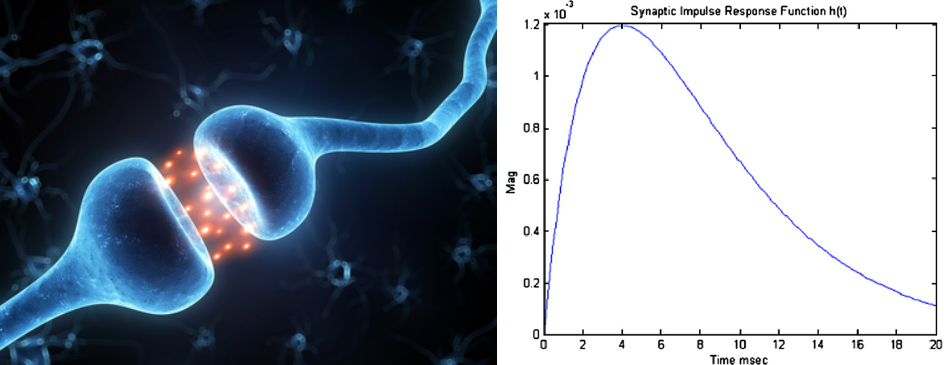
\includegraphics[scale=0.5]{res/synaptischerspalt.png}
\end{figure}
\begin{flalign*}
\text{Präsynaptische Impulsrate}&  \quad \rightarrow \quad  \text{Postsynaptisches Membranpotential}& \\
u_{ein}(t) &\quad \rightarrow \quad  v(t)=h(t)\ast u_{ein}(t) &
\end{flalign*}
\end{frame}

\begin{frame}{Mathematische Realisierung - Neuronenausgang}
\begin{figure}
\centering
\includegraphics[scale=0.21]{res/neuronausgang_sigmoid.png}
\end{figure}

\begin{flalign*}
 \text{Synaptisches Membranpotential}&  \quad \rightarrow \quad  \text{Impulsrate}& \\
v(t) &\quad \rightarrow \quad  u_{aus}(t)=S(v(t)) &
\end{flalign*}
\end{frame}

\begin{frame}{Experimente - Vergleich fMRI- mit EEG-Modell}
\begin{figure}
\centering
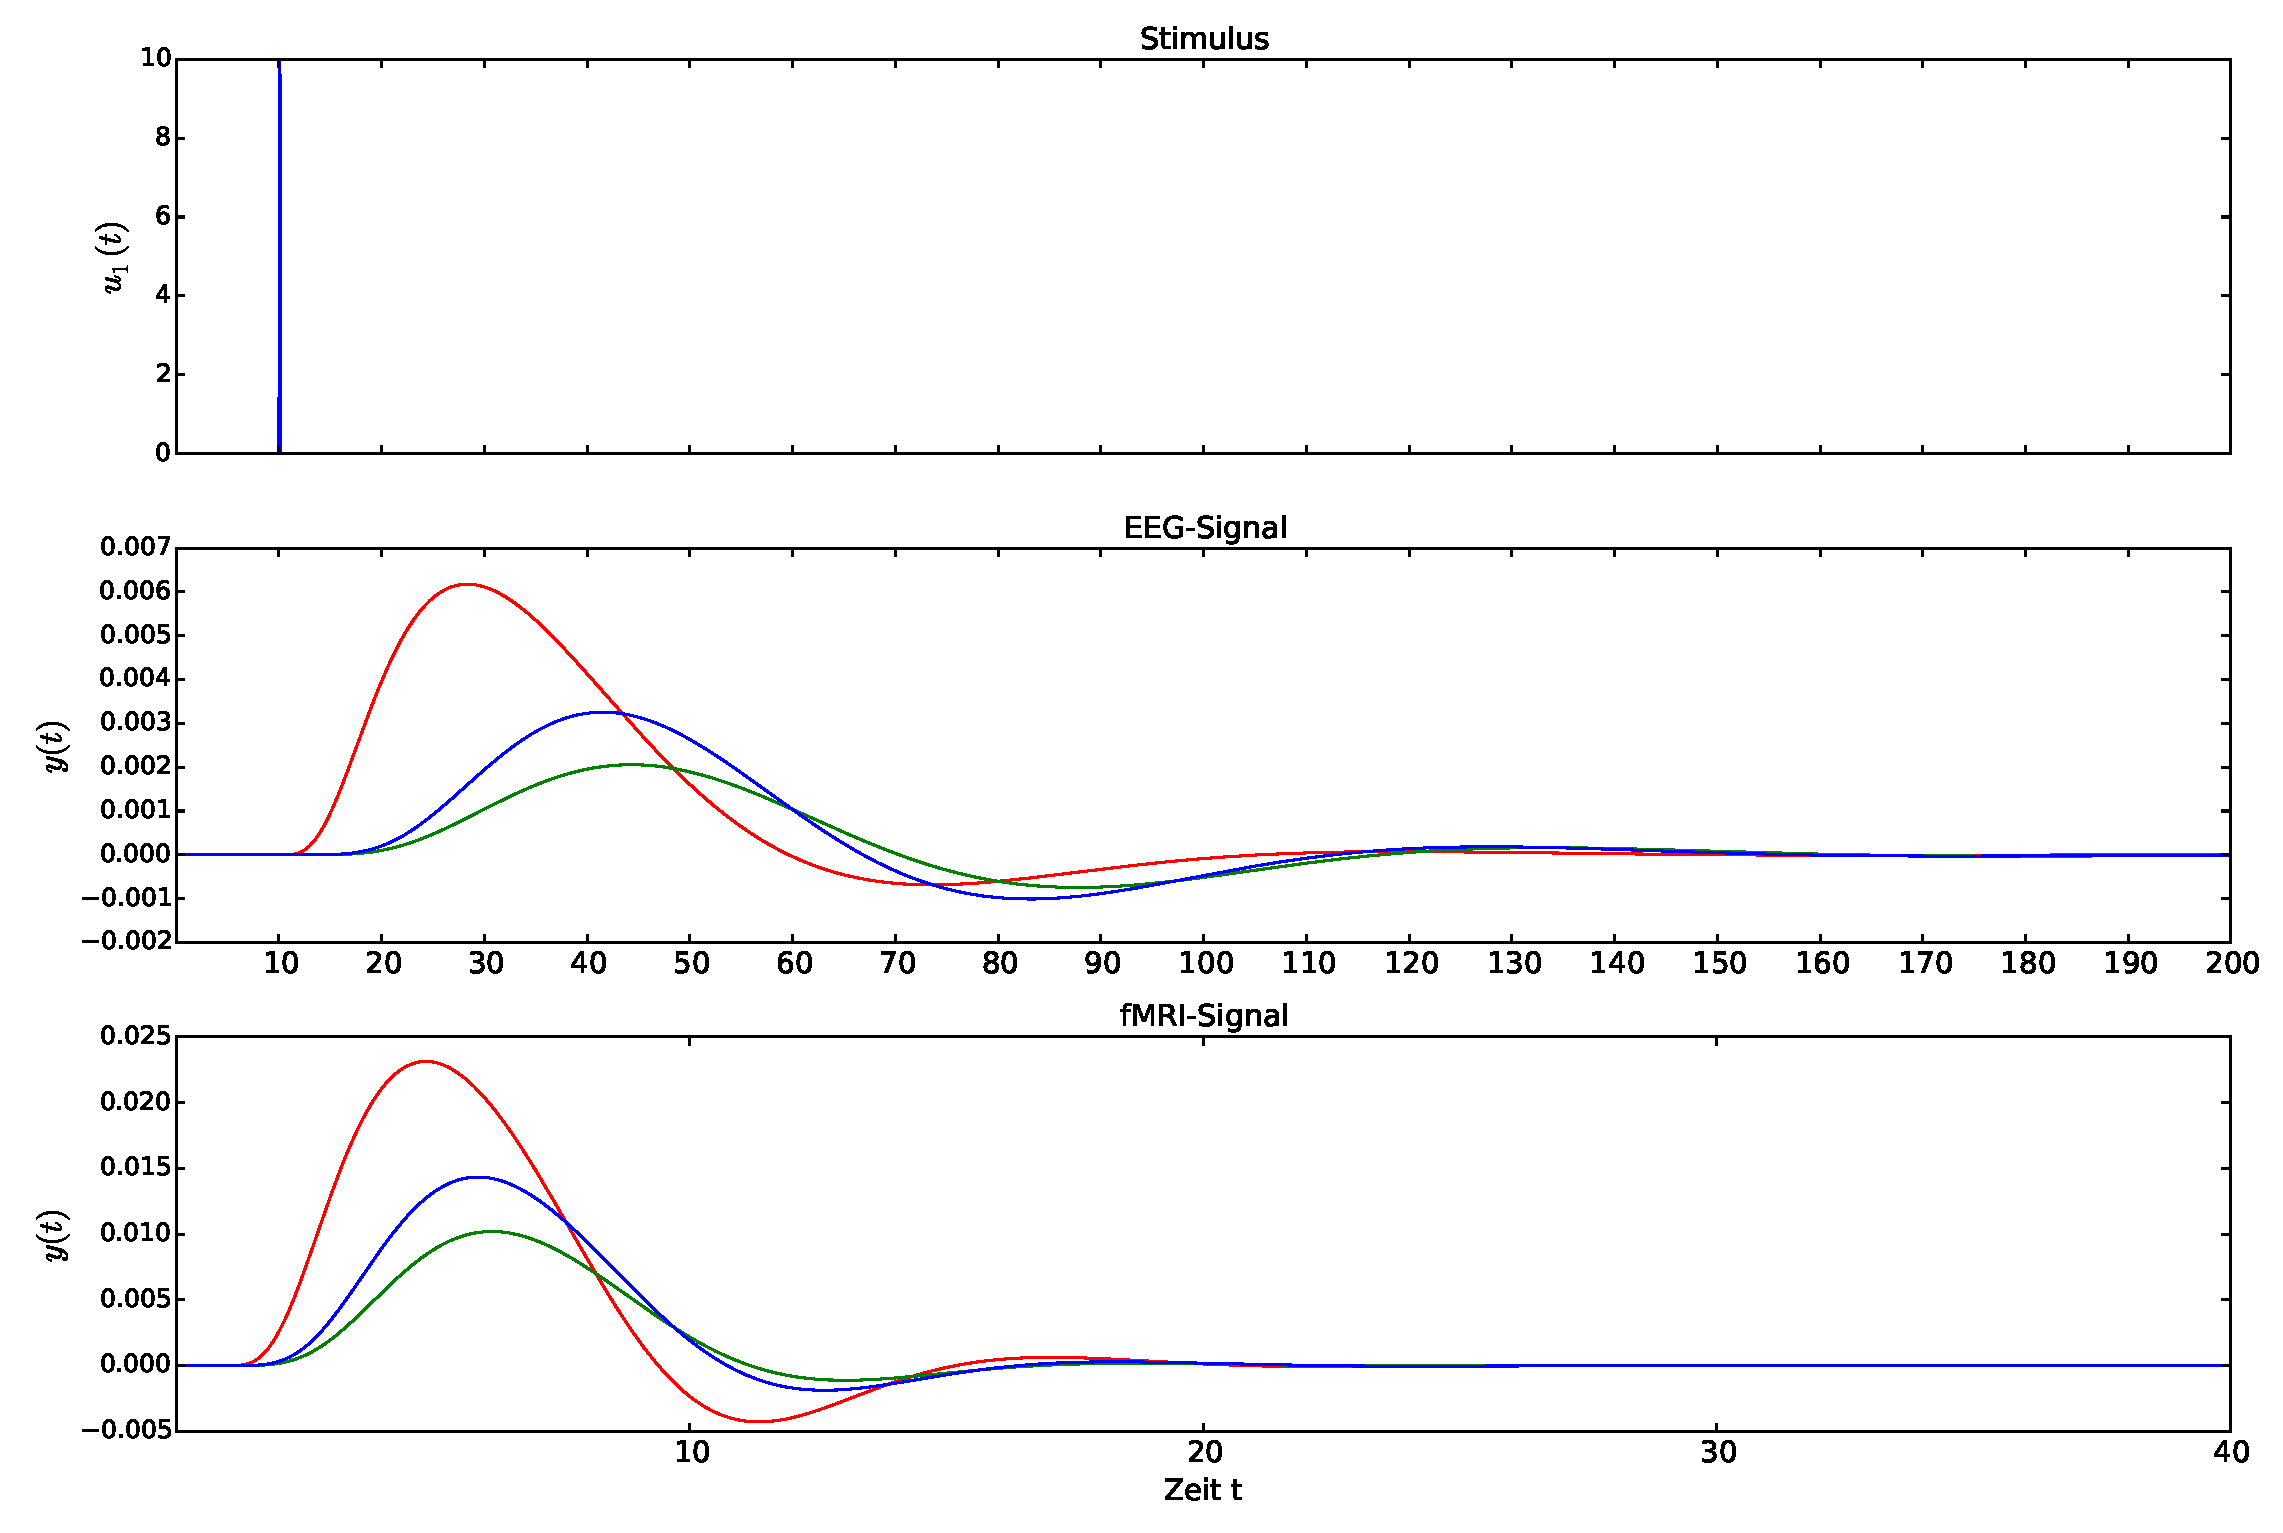
\includegraphics[scale=0.25]{res/hemo-EEG-vergleich.eps}
\end{figure}
\end{frame}

\begin{frame}{Experimente - Vergleich fMRI- mit EEG-Modell}
\begin{figure}
\centering
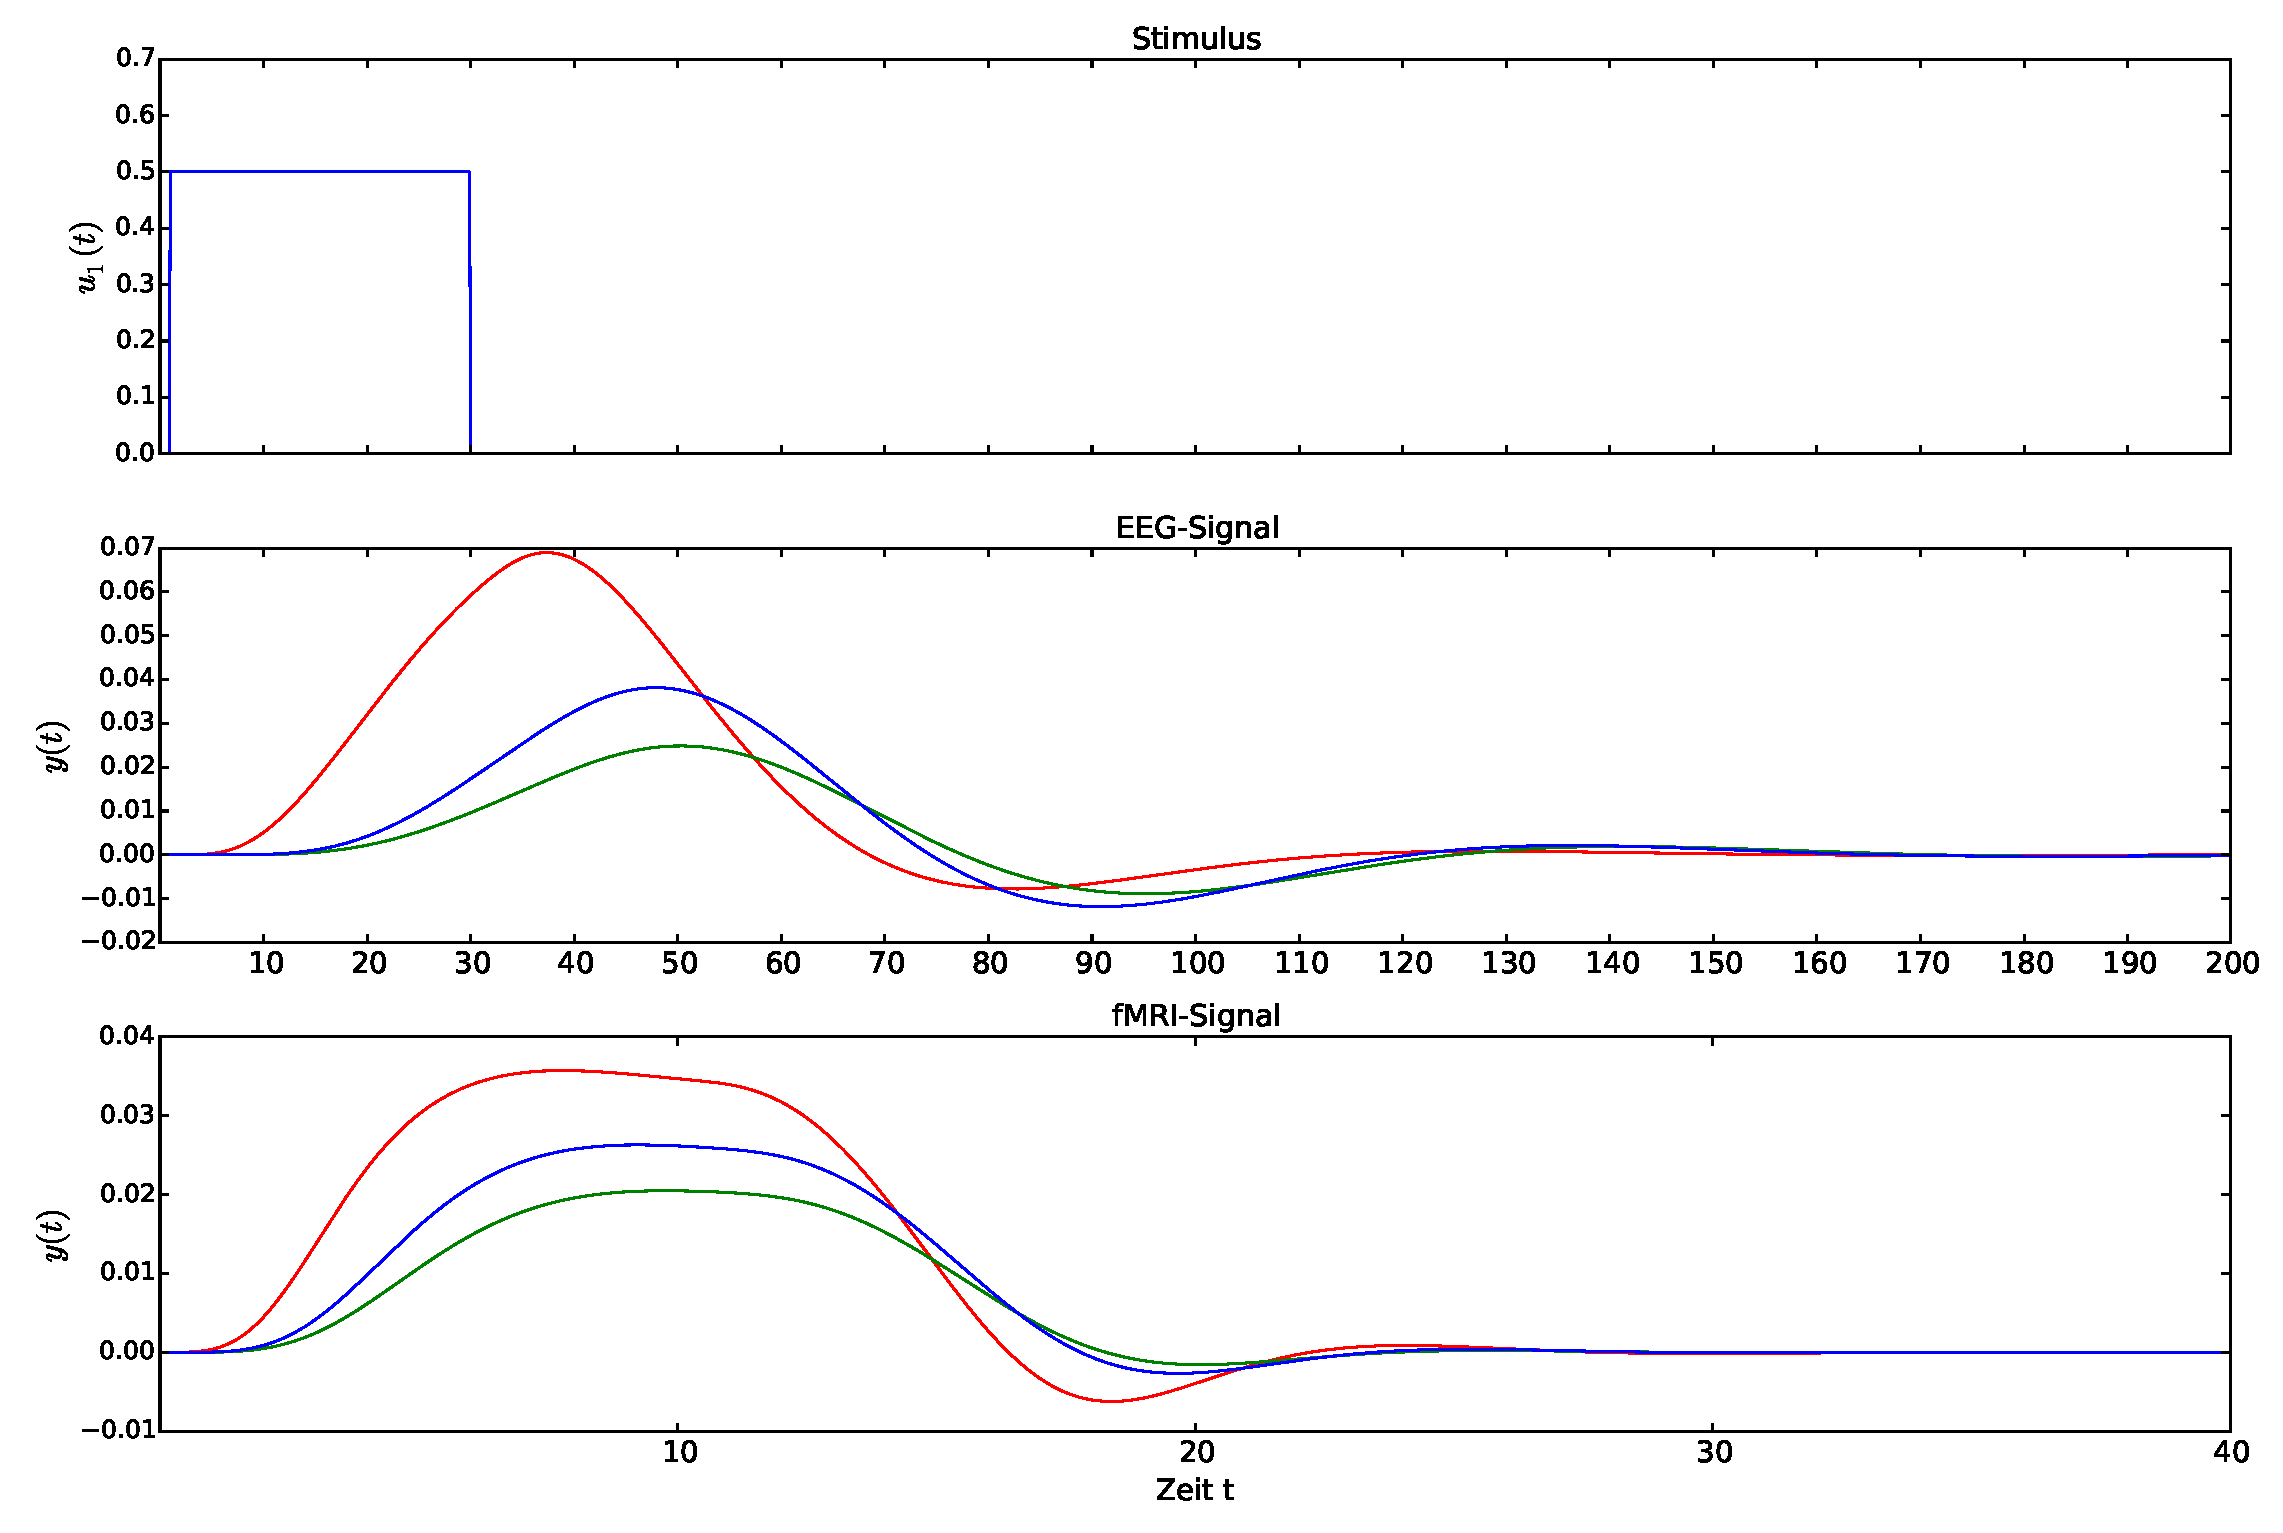
\includegraphics[scale=0.25]{res/hemo-EEG-vergleich2.eps}
\end{figure}
\end{frame}

\begin{frame}{Experimente - Vergleich fMRI- mit EEG-Modell}
\begin{figure}
\centering
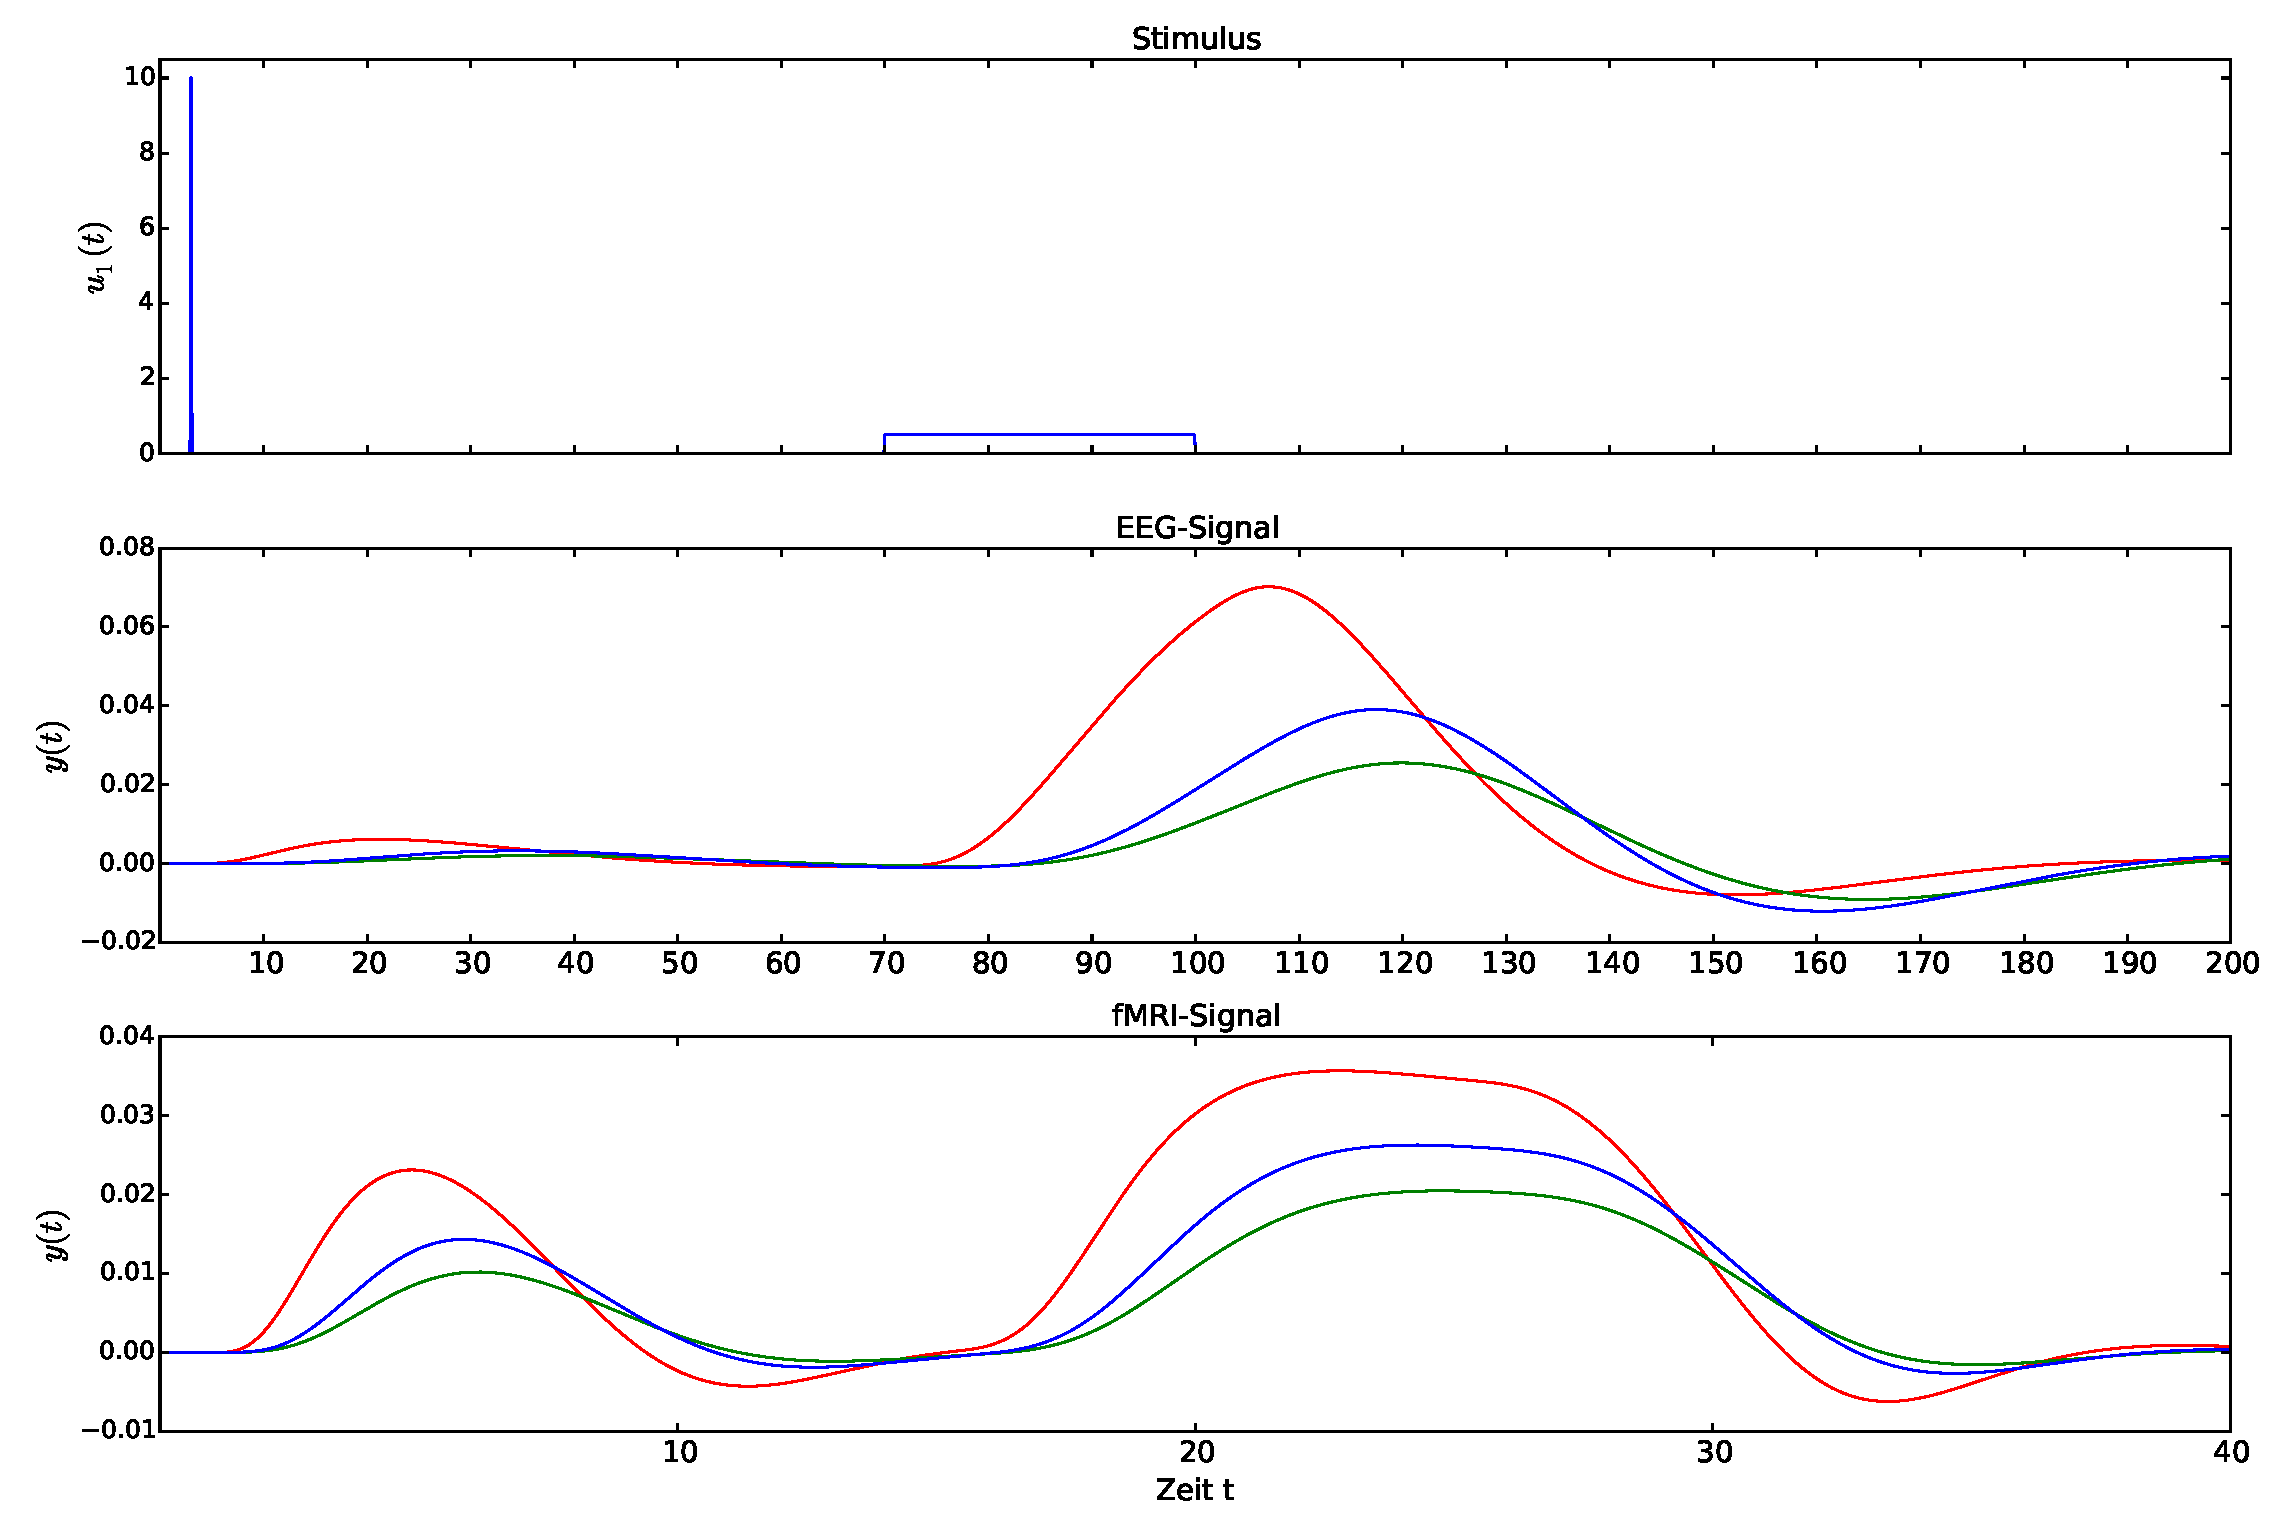
\includegraphics[scale=0.25]{res/hemo-EEG-vergleich3.eps}
\end{figure}
\end{frame}
 
\begin{frame}{Zusammenfassung}	
 \end{frame}

\section{Literatur}
	\begin{frame}{Literatur}
		\begin{itemize}
			\item \textit{Dynamic causal modelling} \\ {\small K.J. Friston, L. Harrison and W. Penny / NeuroImage \textbf{4} (2003)} \\ {\footnotesize \url{web.mit.edu/swg/ImagingPubs/connectivity/Dcm_Friston.pdf}}
			\item \textit{Synaptischer Spalt}\\  {\small In: Gedankenschatz: Bewusstsein- und Persönlichkeitsentfaltung}\\{\footnotesize \url{http://gedankenschatz.de/quantenphysik-im-kopf/}}  {\tiny(Abgerufen: 6. Juli 2016, 12:28 UTC)}
			\item \textit{Sternneuronen}\\{\footnotesize \url{http://gdpsychtech.blogspot.de/2014/06/medium-spiny-neurons-msn.html}}  {\tiny(Abgerufen: 6. Juli 2016, 12:28 UTC)}	
						
											%20Amine/artikel_biogene%20amine.html
			%\url{https://de.wikipedia.org/wiki/Funktionelle_Magnetresonanztomographie} 
%			\item \textit{{\small Bayesian Estimation of Dynamical Systems: An Application to fMRI}} \\ {\small K.J. Friston / NeuroImage (2002)} \\ {\footnotesize \url{www.sciencedirect.com/science/article/pii/S1053811901910444}}
		\end{itemize}
	\end{frame}
	
	\begin{frame}{Literatur}
		\begin{itemize}
			\item \textit{Pyramidenzellen}\\{\footnotesize \url{http://www.ruf.rice.edu/~lngbrain/Sidhya/}}  {\tiny(Abgerufen: 6. Juli 2016, 12:28 UTC)}	
			\item \textit{Aktionspotential und Neurotransmission}\\{\small In: Institut for complex Systems, Forschungszentrum Jülich}\\{\footnotesize \url{http://www.fz-juelich.de/ics/ics-4/DE/Forschungsthemen/02Biogene}}  {\tiny(Abgerufen: 6. Juli 2016, 12:28 UTC)}
			\item \textit{EEG and ERP Laboratory Experiment Demonstration}\\{\footnotesize \url{http://jerlab.psych.sc.edu/infantdevelopmentlab/pwreegdemobaby/pwrbabydemo1.htm}}  {\tiny(Abgerufen: 6. Juli 2016, 12:28 UTC)}
		\end{itemize}
	\end{frame}
\end{document}
